\documentclass{extbook}[14pt]
\usepackage{multicol, enumerate, enumitem, hyperref, color, soul, setspace, parskip, fancyhdr, amssymb, amsthm, amsmath, bbm, latexsym, units, mathtools}
\everymath{\displaystyle}
\usepackage[headsep=0.5cm,headheight=0cm, left=1 in,right= 1 in,top= 1 in,bottom= 1 in]{geometry}
\usepackage{dashrule}  % Package to use the command below to create lines between items
\newcommand{\litem}[1]{\item #1

\rule{\textwidth}{0.4pt}}
\pagestyle{fancy}
\lhead{}
\chead{Answer Key for Makeup Progress Quiz -1 Version B}
\rhead{}
\lfoot{7547-2949}
\cfoot{}
\rfoot{Fall 2020}
\begin{document}
\textbf{This key should allow you to understand why you choose the option you did (beyond just getting a question right or wrong). \href{https://xronos.clas.ufl.edu/mac1105spring2020/courseDescriptionAndMisc/Exams/LearningFromResults}{More instructions on how to use this key can be found here}.}

\textbf{If you have a suggestion to make the keys better, \href{https://forms.gle/CZkbZmPbC9XALEE88}{please fill out the short survey here}.}

\textit{Note: This key is auto-generated and may contain issues and/or errors. The keys are reviewed after each exam to ensure grading is done accurately. If there are issues (like duplicate options), they are noted in the offline gradebook. The keys are a work-in-progress to give students as many resources to improve as possible.}

\rule{\textwidth}{0.4pt}

\begin{enumerate}\litem{
Describe the end behavior of the polynomial below.
\[ f(x) = -9(x + 4)^{3}(x - 4)^{6}(x + 5)^{2}(x - 5)^{3} \]

The solution is the graph below, which is option B.
\begin{center}
    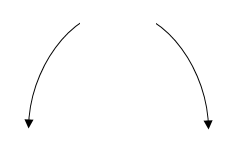
\includegraphics[width=0.3\textwidth]{../Figures/polyEndBehaviorBB.png}
\end{center}\begin{enumerate}[label=\Alph*.]
\begin{multicols}{2}
\item 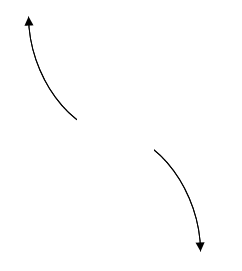
\includegraphics[width = 0.3\textwidth]{../Figures/polyEndBehaviorAB.png}
\item 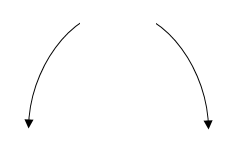
\includegraphics[width = 0.3\textwidth]{../Figures/polyEndBehaviorBB.png}
\item 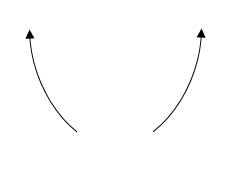
\includegraphics[width = 0.3\textwidth]{../Figures/polyEndBehaviorCB.png}
\item 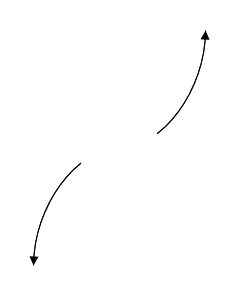
\includegraphics[width = 0.3\textwidth]{../Figures/polyEndBehaviorDB.png}
\end{multicols}\item None of the above.\end{enumerate}
\textbf{General Comment:} Remember that end behavior is determined by the leading coefficient AND whether the \textbf{sum} of the multiplicities is positive or negative.
}
\litem{
Describe the zero behavior of the zero $x = 2$ of the polynomial below.
\[ f(x) = 9(x + 4)^{6}(x - 4)^{4}(x - 2)^{9}(x + 2)^{6} \]

The solution is the graph below, which is option D.
\begin{center}
    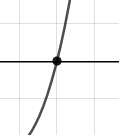
\includegraphics[width=0.3\textwidth]{../Figures/polyZeroBehaviorCopyDB.png}
\end{center}\begin{enumerate}[label=\Alph*.]
\begin{multicols}{2}
\item 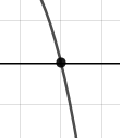
\includegraphics[width = 0.3\textwidth]{../Figures/polyZeroBehaviorCopyAB.png}
\item 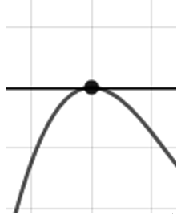
\includegraphics[width = 0.3\textwidth]{../Figures/polyZeroBehaviorCopyBB.png}
\item 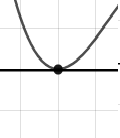
\includegraphics[width = 0.3\textwidth]{../Figures/polyZeroBehaviorCopyCB.png}
\item 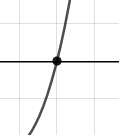
\includegraphics[width = 0.3\textwidth]{../Figures/polyZeroBehaviorCopyDB.png}
\end{multicols}\item None of the above.\end{enumerate}
\textbf{General Comment:} You will need to sketch the entire graph, then zoom in on the zero the question asks about.
}
\litem{
Construct the lowest-degree polynomial given the zeros below. Then, choose the intervals that contain the coefficients of the polynomial in the form $x^3+bx^2+cx+d$.
\[ -5 - 4 i \text{ and } 2 \]

The solution is \( x^{3} +8 x^{2} +21 x -82 \), which is option A.\begin{enumerate}[label=\Alph*.]
\item \( b \in [7, 11], c \in [16.6, 24.7], \text{ and } d \in [-82.5, -81] \)

* $x^{3} +8 x^{2} +21 x -82$, which is the correct option.
\item \( b \in [0, 5], c \in [1.6, 2.3], \text{ and } d \in [-9.2, -7.7] \)

$x^{3} + x^{2} +2 x -8$, which corresponds to multiplying out $(x + 4)(x -2)$.
\item \( b \in [0, 5], c \in [2.8, 4.4], \text{ and } d \in [-11.9, -8.9] \)

$x^{3} + x^{2} +3 x -10$, which corresponds to multiplying out $(x + 5)(x -2)$.
\item \( b \in [-10, -4], c \in [16.6, 24.7], \text{ and } d \in [78.5, 82.4] \)

$x^{3} -8 x^{2} +21 x + 82$, which corresponds to multiplying out $(x-(-5 - 4 i))(x-(-5 + 4 i))(x + 2)$.
\item \( \text{None of the above.} \)

This corresponds to making an unanticipated error or not understanding how to use nonreal complex numbers to create the lowest-degree polynomial. If you chose this and are not sure what you did wrong, please contact the coordinator for help.
\end{enumerate}

\textbf{General Comment:} Remember that the conjugate of $a+bi$ is $a-bi$. Since these zeros always come in pairs, we need to multiply out $(x-(-5 - 4 i))(x-(-5 + 4 i))(x-(2))$.
}
\litem{
Describe the zero behavior of the zero $x = -6$ of the polynomial below.
\[ f(x) = -7(x + 6)^{8}(x - 6)^{9}(x - 3)^{6}(x + 3)^{9} \]

The solution is the graph below, which is option B.
\begin{center}
    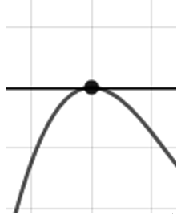
\includegraphics[width=0.3\textwidth]{../Figures/polyZeroBehaviorBB.png}
\end{center}\begin{enumerate}[label=\Alph*.]
\begin{multicols}{2}
\item 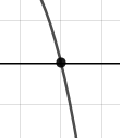
\includegraphics[width = 0.3\textwidth]{../Figures/polyZeroBehaviorAB.png}
\item 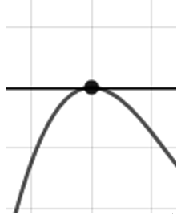
\includegraphics[width = 0.3\textwidth]{../Figures/polyZeroBehaviorBB.png}
\item 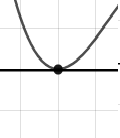
\includegraphics[width = 0.3\textwidth]{../Figures/polyZeroBehaviorCB.png}
\item 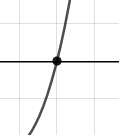
\includegraphics[width = 0.3\textwidth]{../Figures/polyZeroBehaviorDB.png}
\end{multicols}\item None of the above.\end{enumerate}
\textbf{General Comment:} You will need to sketch the entire graph, then zoom in on the zero the question asks about.
}
\litem{
Which of the following equations \textit{could} be of the graph presented below?

\begin{center}
    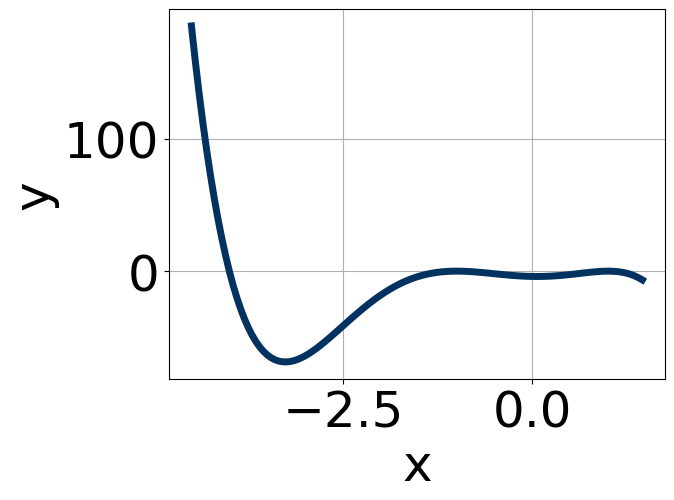
\includegraphics[width=0.5\textwidth]{../Figures/polyGraphToFunctionCopyB.png}
\end{center}




The solution is \( -7(x + 1)^{6} (x - 1)^{6} (x + 4)^{9} \), which is option D.\begin{enumerate}[label=\Alph*.]
\item \( 6(x + 1)^{10} (x - 1)^{6} (x + 4)^{6} \)

The factor $(x + 4)$ should have an odd power and the leading coefficient should be the opposite sign.
\item \( -6(x + 1)^{4} (x - 1)^{5} (x + 4)^{8} \)

The factor $(x - 1)$ should have an even power and the factor $(x + 4)$ should have an odd power.
\item \( -9(x + 1)^{10} (x - 1)^{9} (x + 4)^{11} \)

The factor $(x - 1)$ should have an even power.
\item \( -7(x + 1)^{6} (x - 1)^{6} (x + 4)^{9} \)

* This is the correct option.
\item \( 15(x + 1)^{8} (x - 1)^{4} (x + 4)^{5} \)

This corresponds to the leading coefficient being the opposite value than it should be.
\end{enumerate}

\textbf{General Comment:} General Comments: Draw the x-axis to determine which zeros are touching (and so have even multiplicity) or cross (and have odd multiplicity).
}
\litem{
Which of the following equations \textit{could} be of the graph presented below?

\begin{center}
    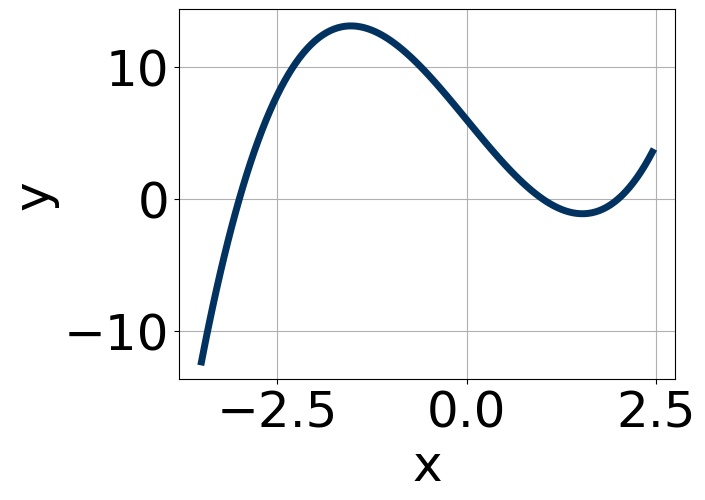
\includegraphics[width=0.5\textwidth]{../Figures/polyGraphToFunctionB.png}
\end{center}




The solution is \( 6(x - 2)^{9} (x + 3)^{9} (x - 1)^{7} \), which is option E.\begin{enumerate}[label=\Alph*.]
\item \( -3(x - 2)^{9} (x + 3)^{11} (x - 1)^{9} \)

This corresponds to the leading coefficient being the opposite value than it should be.
\item \( 17(x - 2)^{10} (x + 3)^{7} (x - 1)^{7} \)

The factor $2$ should have been an odd power.
\item \( -18(x - 2)^{8} (x + 3)^{9} (x - 1)^{5} \)

The factor $(x - 2)$ should have an odd power and the leading coefficient should be the opposite sign.
\item \( 20(x - 2)^{4} (x + 3)^{10} (x - 1)^{9} \)

The factors $2$ and $-3$ have have been odd power.
\item \( 6(x - 2)^{9} (x + 3)^{9} (x - 1)^{7} \)

* This is the correct option.
\end{enumerate}

\textbf{General Comment:} General Comments: Draw the x-axis to determine which zeros are touching (and so have even multiplicity) or cross (and have odd multiplicity).
}
\litem{
Describe the end behavior of the polynomial below.
\[ f(x) = 3(x - 4)^{4}(x + 4)^{5}(x + 3)^{5}(x - 3)^{6} \]

The solution is the graph below, which is option C.
\begin{center}
    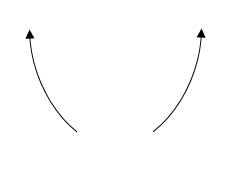
\includegraphics[width=0.3\textwidth]{../Figures/polyEndBehaviorCopyCB.png}
\end{center}\begin{enumerate}[label=\Alph*.]
\begin{multicols}{2}
\item 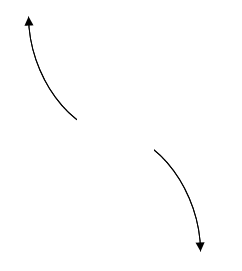
\includegraphics[width = 0.3\textwidth]{../Figures/polyEndBehaviorCopyAB.png}
\item 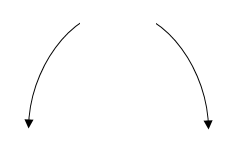
\includegraphics[width = 0.3\textwidth]{../Figures/polyEndBehaviorCopyBB.png}
\item 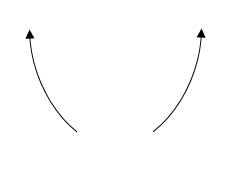
\includegraphics[width = 0.3\textwidth]{../Figures/polyEndBehaviorCopyCB.png}
\item 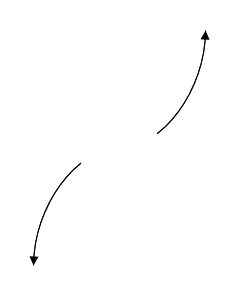
\includegraphics[width = 0.3\textwidth]{../Figures/polyEndBehaviorCopyDB.png}
\end{multicols}\item None of the above.\end{enumerate}
\textbf{General Comment:} Remember that end behavior is determined by the leading coefficient AND whether the \textbf{sum} of the multiplicities is positive or negative.
}
\litem{
Construct the lowest-degree polynomial given the zeros below. Then, choose the intervals that contain the coefficients of the polynomial in the form $ax^3+bx^2+cx+d$.
\[ \frac{6}{5}, \frac{4}{5}, \text{ and } \frac{-5}{2} \]

The solution is \( 50x^{3} +25 x^{2} -202 x + 120 \), which is option B.\begin{enumerate}[label=\Alph*.]
\item \( a \in [50, 56], b \in [225, 228], c \in [298, 302], \text{ and } d \in [113, 124] \)

$50x^{3} +225 x^{2} +298 x + 120$, which corresponds to multiplying out $(5x + 6)(5x + 4)(2x + 5)$.
\item \( a \in [50, 56], b \in [15, 26], c \in [-203, -196], \text{ and } d \in [113, 124] \)

* $50x^{3} +25 x^{2} -202 x + 120$, which is the correct option.
\item \( a \in [50, 56], b \in [140, 148], c \in [0, 13], \text{ and } d \in [-125, -119] \)

$50x^{3} +145 x^{2} +2 x -120$, which corresponds to multiplying out $(5x + 6)(5x -4)(2x + 5)$.
\item \( a \in [50, 56], b \in [15, 26], c \in [-203, -196], \text{ and } d \in [-125, -119] \)

$50x^{3} +25 x^{2} -202 x -120$, which corresponds to multiplying everything correctly except the constant term.
\item \( a \in [50, 56], b \in [-26, -18], c \in [-203, -196], \text{ and } d \in [-125, -119] \)

$50x^{3} -25 x^{2} -202 x -120$, which corresponds to multiplying out $(5x + 6)(5x + 4)(2x -5)$.
\end{enumerate}

\textbf{General Comment:} To construct the lowest-degree polynomial, you want to multiply out $(5x -6)(5x -4)(2x + 5)$
}
\litem{
Construct the lowest-degree polynomial given the zeros below. Then, choose the intervals that contain the coefficients of the polynomial in the form $x^3+bx^2+cx+d$.
\[ -5 + 5 i \text{ and } -1 \]

The solution is \( x^{3} +11 x^{2} +60 x + 50 \), which is option B.\begin{enumerate}[label=\Alph*.]
\item \( b \in [-12, -5], c \in [60, 64], \text{ and } d \in [-51, -40] \)

$x^{3} -11 x^{2} +60 x -50$, which corresponds to multiplying out $(x-(-5 + 5 i))(x-(-5 - 5 i))(x -1)$.
\item \( b \in [7, 18], c \in [60, 64], \text{ and } d \in [48, 53] \)

* $x^{3} +11 x^{2} +60 x + 50$, which is the correct option.
\item \( b \in [-3, 9], c \in [0, 11], \text{ and } d \in [2, 15] \)

$x^{3} + x^{2} +6 x + 5$, which corresponds to multiplying out $(x + 5)(x + 1)$.
\item \( b \in [-3, 9], c \in [-6, -2], \text{ and } d \in [-5, -2] \)

$x^{3} + x^{2} -4 x -5$, which corresponds to multiplying out $(x -5)(x + 1)$.
\item \( \text{None of the above.} \)

This corresponds to making an unanticipated error or not understanding how to use nonreal complex numbers to create the lowest-degree polynomial. If you chose this and are not sure what you did wrong, please contact the coordinator for help.
\end{enumerate}

\textbf{General Comment:} Remember that the conjugate of $a+bi$ is $a-bi$. Since these zeros always come in pairs, we need to multiply out $(x-(-5 + 5 i))(x-(-5 - 5 i))(x-(-1))$.
}
\litem{
Construct the lowest-degree polynomial given the zeros below. Then, choose the intervals that contain the coefficients of the polynomial in the form $ax^3+bx^2+cx+d$.
\[ \frac{-6}{5}, \frac{-1}{2}, \text{ and } \frac{4}{5} \]

The solution is \( 50x^{3} +45 x^{2} -38 x -24 \), which is option E.\begin{enumerate}[label=\Alph*.]
\item \( a \in [40, 53], b \in [43, 50], c \in [-38, -36], \text{ and } d \in [20, 26] \)

$50x^{3} +45 x^{2} -38 x + 24$, which corresponds to multiplying everything correctly except the constant term.
\item \( a \in [40, 53], b \in [-133, -118], c \in [93, 99], \text{ and } d \in [-28, -21] \)

$50x^{3} -125 x^{2} +98 x -24$, which corresponds to multiplying out $(5x -6)(2x -1)(5x -4)$.
\item \( a \in [40, 53], b \in [-78, -71], c \in [-6, 0], \text{ and } d \in [20, 26] \)

$50x^{3} -75 x^{2} -2 x + 24$, which corresponds to multiplying out $(5x -6)(2x + 1)(5x -4)$.
\item \( a \in [40, 53], b \in [-54, -41], c \in [-38, -36], \text{ and } d \in [20, 26] \)

$50x^{3} -45 x^{2} -38 x + 24$, which corresponds to multiplying out $(5x -6)(2x -1)(5x + 4)$.
\item \( a \in [40, 53], b \in [43, 50], c \in [-38, -36], \text{ and } d \in [-28, -21] \)

* $50x^{3} +45 x^{2} -38 x -24$, which is the correct option.
\end{enumerate}

\textbf{General Comment:} To construct the lowest-degree polynomial, you want to multiply out $(5x + 6)(2x + 1)(5x -4)$
}
\end{enumerate}

\end{document}